\clearpage
\chapter{Experiments}
Chapter 3 described how the experiments are to be executed and Chapter 4 described the subjects of the tests, algorithms and software. This chapter contains the results of these experiments. Each of the sections will contain graphs and tables showcasing the results, alongside a brief description of the numbers produced. 

\section{Quicksort}
\label{sec: QuickSort}
Quicksort experiments were conducted with 3 sizes of arrays, 6 implementations and 2 .NET environment version (Tab. \ref{tab:QuicksortParameters}). 

.NET version had significant impact on functional implementation of the algortihm. Functional version showed average of $\approx 27\%$ improvement (Fig. \ref{fig:47vsCoreFunc1000000}) on .NET Core 3.1, while the imperative smaller but still significant  $\approx 9\%$ (Fig. \ref{fig:47vsCoreImp1000000}).

Async-await version performed worse in all scenarios. Functional version was slower on average by $\approx 54\%$, while the imperative by dramatic $\approx 96\%$. These relations where consistent across all array sizes and version, slightly favouring .NET Core 3.1. (Tab. \ref{tab: QuicksortBenchmarking}).

The optimized parallel versions with depth control performed significantly better. LINQ version gained average reduction  of $\approx 45\%$ while the imperative one 
$\approx 21\%$. Here difference between .NET version was more pronounced. A difference of 4 percentage points for the functional one (43\% -> 47\%) and 7 percentage points for the imperative one (18\% -> 25\%). (Tab. \ref{tab: QuicksortBenchmarking}).

Imperative version of quick sort algorithm performer better than the functional one. On average it was faster by $\approx 95\%$ on .NET Framework 4.7 and $\approx 91\%$ on .NET Core 3.1 (Fig \ref{fig:FuncVsImp1000000}).

Memory consumption increased in both versions. Functional parallel version consumed $\approx 17\%$ more memory by average. Imperative parallel version increased it $\approx 73\%$. This was consistent among the .NET versions but consumption increased less the bigger the sorted array was (Tab. \ref{tab: QuicksortBenchmarking}).


\begin{table}[!ht]
    \centering
    \caption{Quicksort benchmarking parameters}
		\label{tab:QuicksortParameters}
    \begin{tabular}{p{3cm}p{4cm}}
			\toprule
			\bfseries Name 	&
			\bfseries Value \\
			\midrule
			Small array & 10000  \\
			Medium array & 100000 \\
			Large array & 1000000 \\
			Old version & .NET Framework 4.7 \\ 
			Modern version & .NET Core 3.1 \\ 
			\bottomrule
    \end{tabular}
\end{table}

\begin{figure}[htb]
\centering
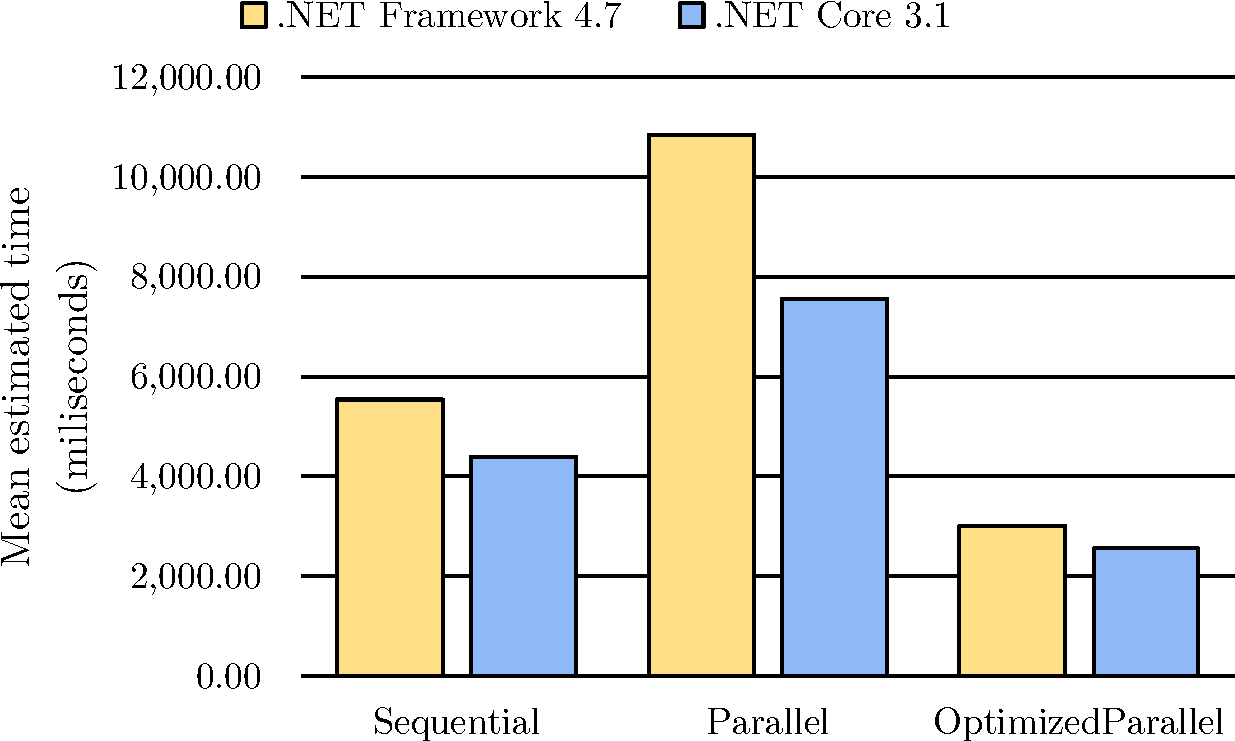
\includegraphics[width=.8\linewidth]{figures04/47vsCoreFunc1000000.pdf}
\caption{Difference between .NET versions in functional implementation - large array}
\label{fig:47vsCoreFunc1000000}
\end{figure}

\begin{figure}[htb]
\centering
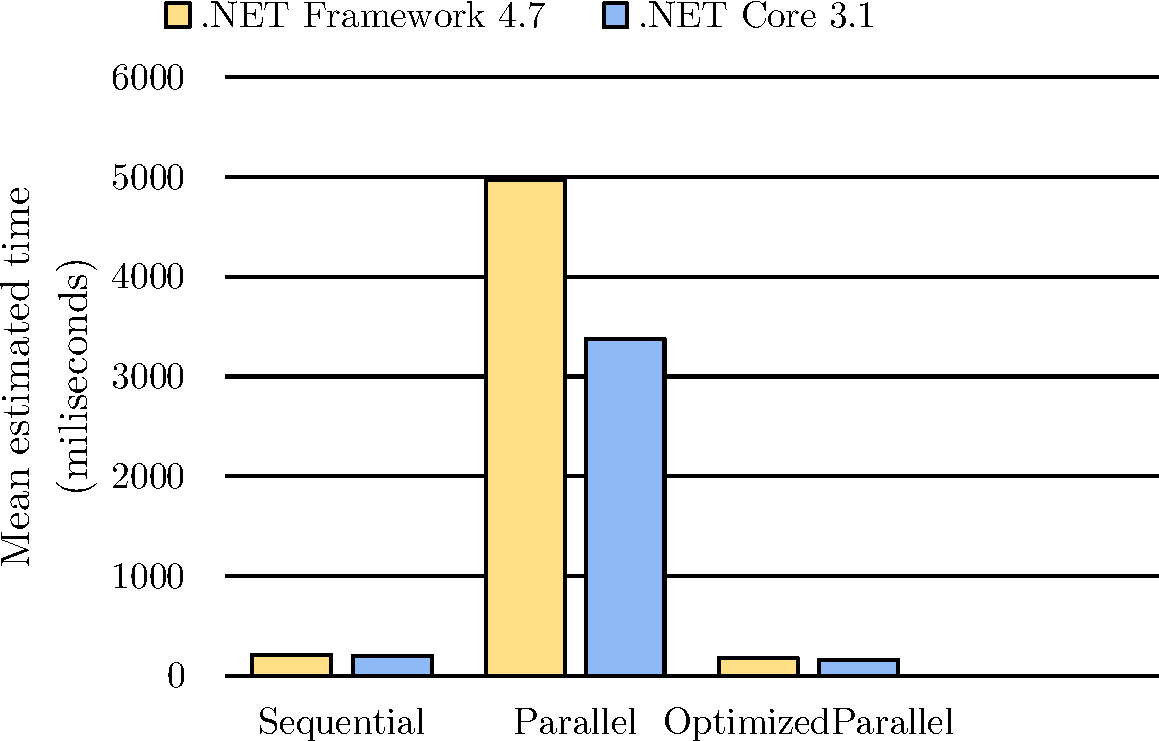
\includegraphics[width=.8\linewidth]{figures04/47vsCoreImp1000000.pdf}
\caption{Difference between .NET versions in imperative implementation - large array}
\label{fig:47vsCoreImp1000000}
\end{figure}

\begin{figure}[htb]
\centering
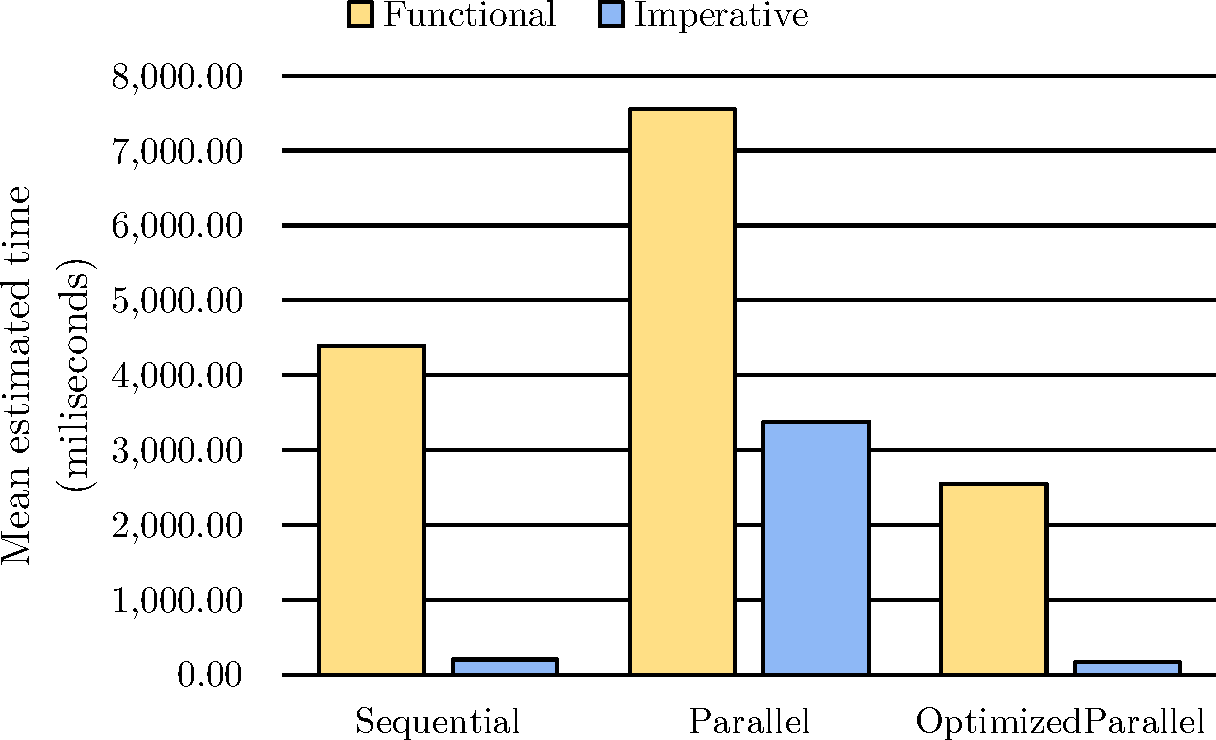
\includegraphics[width=.8\linewidth]{figures04/FuncVsImp1000000.pdf}
\caption{Performance across all version with large array on .NET Core}
\label{fig:FuncVsImp1000000}
\end{figure}

\begin{table}\footnotesize
    \centering
    \caption{Quicksort benchmarking results}
		\label{tab: QuicksortBenchmarking}
    \begin{tabularx}{\linewidth}{Xrrrrrrrr} 
		  \toprule
			\toprule
			\bfseries Version 		&
			\bfseries N    	    	& 
			\bfseries Mean 	      &
			\bfseries Error       &
			\bfseries StdDev 	    &
			\bfseries Gen 0	    	&
			\bfseries Gen 1	    	&
			\bfseries Gen 2	    	&
			\bfseries Alloc.      \\ 
			&
			&
			\bfseries {[}ms{]} &
			\bfseries {[}ms{]} &
			\bfseries {[}ms{]} &
			&
			&
			&
			\bfseries{[}MB{]} \\			
			\midrule 
			\multicolumn{9}{c}{.NET Framework 4.7} \\ 
			\midrule 
SequentialFunctional	&	10000	&	31.39	&	0.13	&	0.11	&	2906	&	594	&	250	&	17	\\
ParallelFunctional	&	10000	&	85.54	&	0.52	&	0.43	&	4500	&	500	&	167	&	26	\\
OptimizedParallelFunctional	&	10000	&	16.44	&	0.33	&	0.29	&	4000	&	1000	&	0	&	22	\\
SequentialImperative	&	10000	&	0.83	&	0.00	&	0.00	&	83	&	41	&	0	&	0.509	\\
ParallelImperative	&	10000	&	51.13	&	0.97	&	2.21	&	2364	&	364	&	91	&	8	\\
OptimizedParallelImperative	&	10000	&	0.69	&	0.01	&	0.01	&	410	&	203	&	0	&	3	\\
SequentialFunctional	&	100000	&	438.21	&	6.95	&	5.81	&	35000	&	9000	&	2000	&	201	\\
ParallelFunctional	&	100000	&	950.50	&	11.81	&	11.05	&	51000	&	11000	&	2000	&	287	\\
OptimizedParallelFunctional	&	100000	&	265.64	&	6.11	&	15.33	&	40000	&	9000	&	1000	&	242	\\
SequentialImperative	&	100000	&	14.39	&	0.14	&	0.13	&	844	&	375	&	141	&	5	\\
ParallelImperative	&	100000	&	488.38	&	4.33	&	4.05	&	49000	&	0	&	0	&	84	\\
OptimizedParallelImperative	&	100000	&	11.20	&	0.46	&	0.56	&	6063	&	781	&	250	&	19	\\
SequentialFunctional	&	1000000	&	5,548.45	&	69.15	&	57.74	&	368000	&	77000	&	7000	&	2,268	\\
ParallelFunctional	&	1000000	&	10,845.01	&	164.33	&	145.68	&	532000	&	92000	&	4000	&	3,136	\\
OptimizedParallelFunctional	&	1000000	&	3,005.16	&	78.88	&	168.10	&	428000	&	98000	&	5000	&	2,665	\\
SequentialImperative	&	1000000	&	215.68	&	2.12	&	1.98	&	8667	&	3667	&	1000	&	51	\\
ParallelImperative	&	1000000	&	4,970.80	&	41.24	&	36.56	&	496000	&	3000	&	0	&	843	\\
OptimizedParallelImperative	&	1000000	&	184.68	&	4.67	&	12.05	&	67333	&	4667	&	1000	&	149	\\
      \midrule
			\multicolumn{9}{c}{.NET Core 3.1} \\ 
			\midrule 
SequentialFunctional	&	10000	&	23.07	&	0.43	&	0.41	&	1969	&	656	&	219	&	16	\\
ParallelFunctional	&	10000	&	62.52	&	1.21	&	1.73	&	2889	&	667	&	222	&	23	\\
OptimizedParallelFunctional	&	10000	&	12.21	&	0.40	&	1.07	&	2000	&	1000	&	0	&	20	\\
SequentialImperative	&	10000	&	0.83	&	0.01	&	0.01	&	62	&	30	&	0	&	0.508	\\
ParallelImperative	&	10000	&	33.91	&	0.40	&	0.38	&	813	&	375	&	0	&	7	\\
OptimizedParallelImperative	&	10000	&	1.08	&	0.02	&	0.02	&	305	&	152	&	0	&	2	\\
SequentialFunctional	&	100000	&	321.69	&	6.40	&	10.52	&	23000	&	6000	&	1000	&	190	\\
ParallelFunctional	&	100000	&	671.42	&	6.47	&	6.05	&	32000	&	6000	&	1000	&	258	\\
OptimizedParallelFunctional	&	100000	&	157.80	&	5.13	&	13.88	&	29000	&	9000	&	2000	&	226	\\
SequentialImperative	&	100000	&	12.70	&	0.19	&	0.18	&	578	&	297	&	125	&	5	\\
ParallelImperative	&	100000	&	331.97	&	2.57	&	2.14	&	8000	&	0	&	0	&	67	\\
OptimizedParallelImperative	&	100000	&	10.02	&	0.31	&	0.29	&	2469	&	734	&	234	&	19	\\
SequentialFunctional	&	1000000	&	4,397.27	&	63.14	&	59.06	&	259000	&	68000	&	5000	&	2,160	\\
ParallelFunctional	&	1000000	&	7,564.57	&	85.35	&	79.84	&	343000	&	77000	&	4000	&	2,840	\\
OptimizedParallelFunctional	&	1000000	&	2,555.12	&	67.87	&	72.62	&	303000	&	85000	&	3000	&	2,520	\\
SequentialImperative	&	1000000	&	206.51	&	1.29	&	1.14	&	6667	&	3667	&	1000	&	51	\\

			\bottomrule
    \end{tabularx}
\end{table}

\clearpage
\section{K-means clustering}
\label{sec: K-means}
K-means clustering algorithm experiments were conducted using \emph{White 
wine quality} dataset \cite{WhiteWine}. Sequential version of the algorithm 
had MET $\approx 2.45s$ while the parallel one had MET $\approx 0.5s$, for a $
\approx 80\%$ reduction at the cost of $\approx 18\%$ increase of memory 
consumption. Using partitioner further dropped down the MET to $\approx 0.43s$
 which is a $\approx 82\%$ reduction from the sequential version and $\approx 
15\%$ from the parallel one with equal memory consumption increase (Fig. \ref{fig: KMeansPerformance}, Fig. \ref{fig: KMeansMemory}, Tab. \ref{tab: 
KMeansBenchmarking}).

\begin{figure}[htb]
\centering
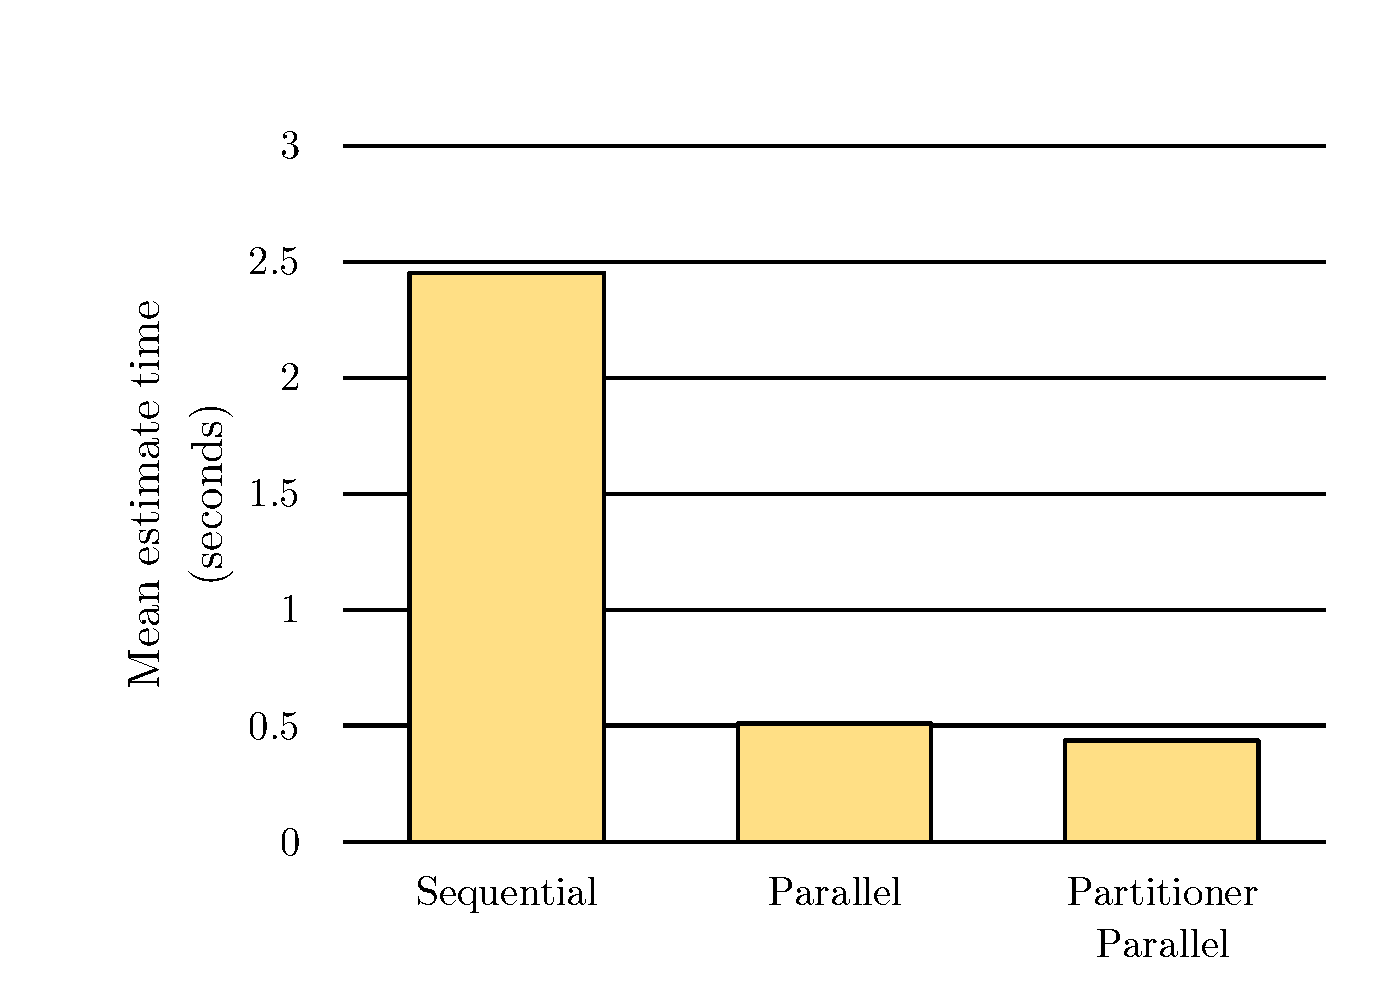
\includegraphics[width=.8\linewidth]{figures04/KMeans.pdf}
\caption{K-means clustering  performance}
\label{fig: KMeansPerformance}
\end{figure}

\begin{figure}[htb]
\centering
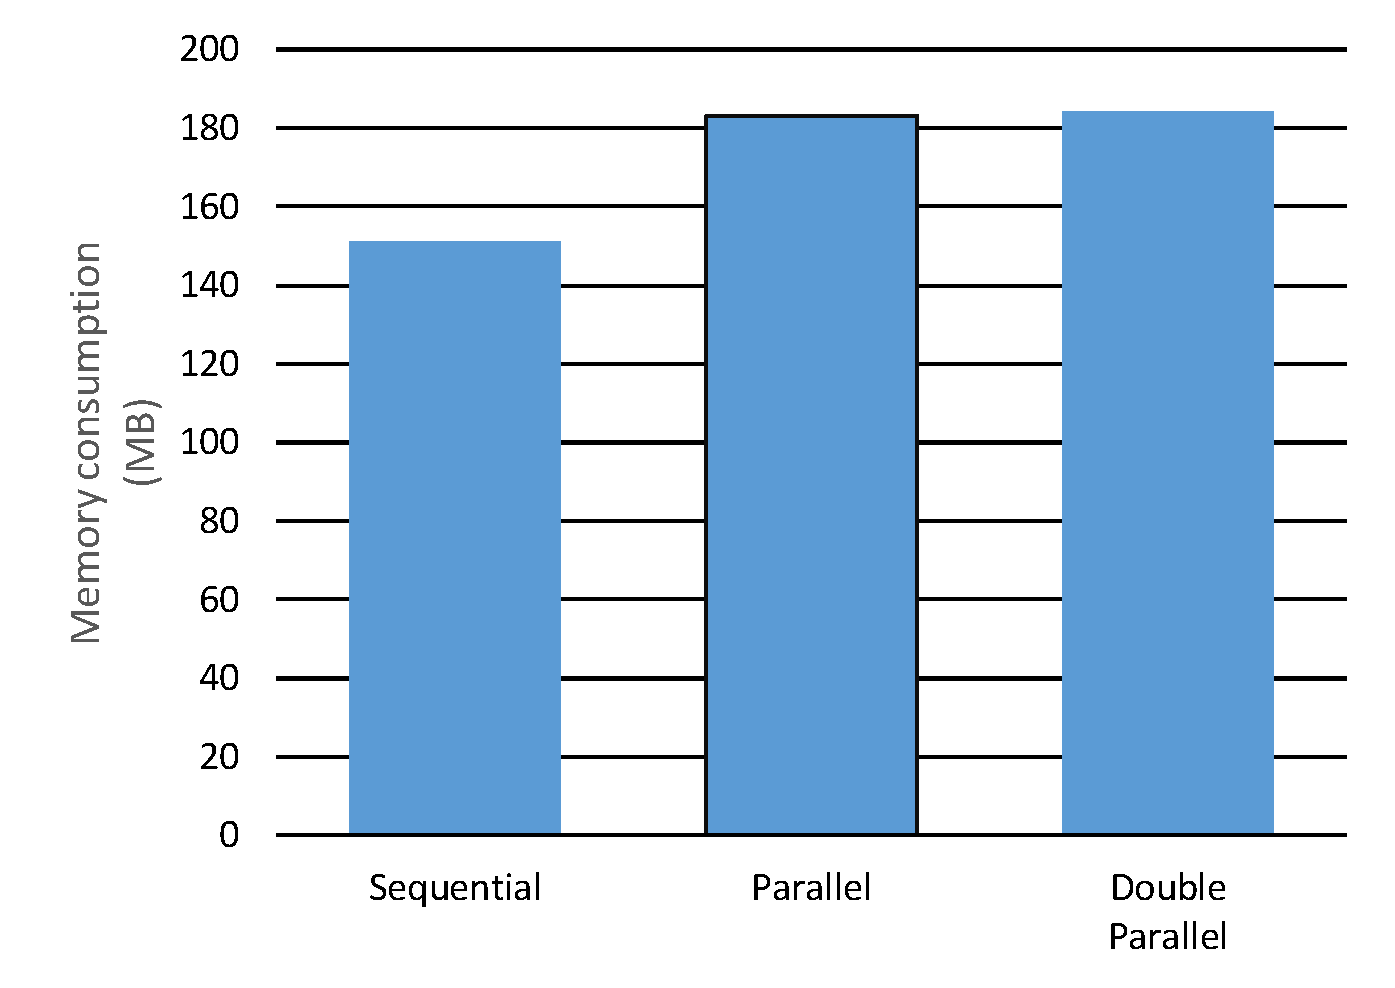
\includegraphics[width=.8\linewidth]{figures04/KMeansMemory.pdf}
\caption{K-means clustering memory consumption}
\label{fig: KMeansMemory}
\end{figure}

\begin{table}[ht]%\small
    \centering
    \caption{K-means clustering benchmarking results}
		\label{tab: KMeansBenchmarking}
    \begin{tabularx}{\linewidth}{Xrrrrrrr} 
		\toprule
		\toprule
			\bfseries Version 		&
			\bfseries Mean 	      &
			\bfseries Error       &
			\bfseries StdDev 	    &
			\bfseries Gen 0	    	&
			\bfseries Gen 1	    	&
			\bfseries Gen 2	    	&
			\bfseries Alloc.      \\ 
			&
			\bfseries {[}ms{]} &
			\bfseries {[}ms{]} &
			\bfseries {[}ms{]} &
			&
			&
			&
			\bfseries{[}MB{]} \\	
			\midrule 
Sequential & 2,453.7 	& 25.01	& 20.89	& 18000 & 	2000 & 	0 & 151  \\
Parallel & 509.6 	& 8.28 	& 8.50 	& 23000 & 	9000 & 	0 & 183  \\ 
PartitionerParallel & 434.5 	& 2.69 	& 2.52 	& 23000 & 	8000 & 	0 & 184  \\
			\bottomrule
		\end{tabularx}
\end{table}

\clearpage
\section{Mandelbrot}
\label{sec: Mandelbrot}
Mandelbrot algorithm experiments were conducted using parameters presented in 
Tab. \ref{tab: MandelbrotParameters}. They describe amount of pixels 
generated and bitmap dimensions.
Sequential version of the algorithm had a MET  $\approx 5.6s$ . Parallel 
counterpart clocked at MET  $\approx 2.1s$, for a $\approx 62\%$ reduction. 
Parallel version with two \emph{Parallel.For} loops had a MET $\approx 2.7s$ 
which is $\approx 21\%$ slower than the less parallelized version using only 
one parallel loop. The best performing version using value type complex 
number had MET $\approx 1.9s$, for a $\approx 66\%$  reduction compared to 
sequential version and $\approx 11\%$  reduction to the parallel version. 
Additionaly, the value type version had 0 GC clean ups and virtually no (
compared to others) memory consumption (Fig. \ref{fig: MandelbrotPerformance}
, Tab. \ref{tab: MandelbrotBenchmarking}).

\begin{table}[!ht]
    \centering
    \caption{Mandelbrot benchmarking experiment parameters}
		\label{tab: MandelbrotParameters}
    \begin{tabular}{p{3cm}p{3cm}}
			\toprule
			\bfseries Name 	&
			\bfseries Value \\
			\midrule
			Width & 2.5 \\
			Height & 2.5 \\
			Column amount & 4000 \\ 
			Row amount  & 4000 \\	
			\bottomrule
    \end{tabular}
\end{table}

\begin{figure}[htb]
\centering
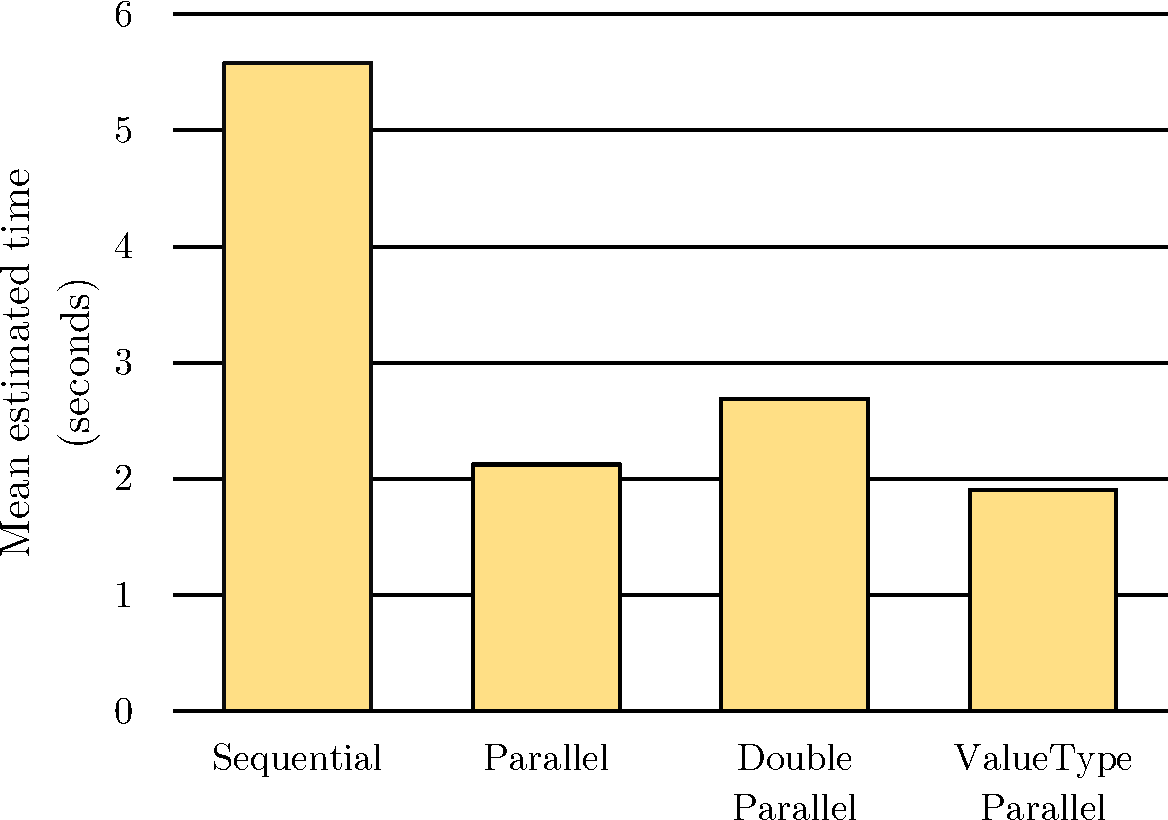
\includegraphics[width=.8\linewidth]{figures04/Mandelbrot.pdf}
\caption{Mandelbrot algorithm performance}
\label{fig: MandelbrotPerformance}
\end{figure}

\begin{table}[ht]%\small
    \centering
    \caption{Mandelbrot benchmarking results}
		\label{tab: MandelbrotBenchmarking}
    \begin{tabularx}{\linewidth}{Xrrrrrrr}
		  \toprule
			\toprule
			\bfseries Version 		&
			\bfseries Mean 	      &
			\bfseries Error       &
			\bfseries StdDev 	    &
			\bfseries Gen 0	    	&
			\bfseries Gen 1	    	&
			\bfseries Gen 2	    	&
			\bfseries Alloc.      \\ 
			&
			\bfseries {[}s{]} &
			\bfseries {[}s{]} &
			\bfseries {[}s{]} &
			&
			&
			&
			\bfseries{[}MB{]} \\			
			\midrule 
			Sequential & 5.576 & 0.0564 & 0.0528 & 2483000 & 1000 & 1000 & 19851  \\ 
			Parallel & 2.120 & 0.0458 & 0.1350 & 2485000 & 6000 & 1000 & 19843 \\ 
			DoubleParallel & 2.684 & 0.0553 & 0.1632 & 2487000 & 39000 & 2000 & 19852  \\ 
			ValueTypeParallel & 1.903 & 0.0137 & 0.0128 & 0 & 0 & 0 & 46  \\ 
			\bottomrule
	\end{tabularx}
\end{table}

\clearpage
\label{sec: NuGet}
\section{NuGet package ranking}
NuGet package ranking software was tested using 3 datasets varying in size, 
other parameters were constast across tests (Tab. \ref{tab: NuGetParameters})
. \\
When testing with the small dataset, sequential version had MET $\approx 1.7s$
, while parallel one had MET $\approx 0.35s$ for a $\approx 79\%$ reduction. 
In this case, usage of partitioner worsened the performance with MET  $\approx
 0.38s$, which is $\approx 6\%$ slower (Fig. \ref{fig: NugetPerfSmall}). \\ 
During tests with the medium dataset, sequential version had MET $\approx 17.5
s$. Parallel version clocket at $\approx 4.6s$, for a $\approx 76\%$ 
reduction. This time partitioner version improved the performance at MET $
\approx 3s$, which is $\approx 35\%$ faster than the bare parallel 
counterpart (Fig. \ref{fig: NugetPerfMed}). \\ 
Finally sequential version on the large dataset had MET $\approx 56.9s$ while 
the parallel one had MET $\approx 14.4s$ which is $\approx 75\%$ less.
The partitioner continued the reducing trend at MET $\approx 9.4s$, improving 
the parallel version by $\approx 42 \%$ (Fig. \ref{fig: NugetPerfLarge}). \\
Across all dataset the parallel version observed increase of memory 
consumption of $\approx 14\%$ (Fig. \ref{fig: NugetMemory}) (Tab. \ref{tab: NugetBenchmarking}).

\begin{table}[!ht]
    \centering
    \caption{Nuget package ranking experiments parameters}
		\label{tab: NuGetParameters}
    \begin{tabular}{p{5cm}p{3cm}}
			\toprule
			\bfseries Name 	&
			\bfseries Value \\
			\midrule
			\emph{Map} degree of parallelism & 10 \\
			\emph{Reduce} degree of parallelism & 10 \\
			Iterations & 10 \\ 
			Small dataset  & 1000 packages  \\	
			Medium dataset  & 5000 packages  \\	
			Large dataset  & 10000 packages  \\	
			\bottomrule
    \end{tabular}
\end{table}

\begin{figure}[htb]
\centering
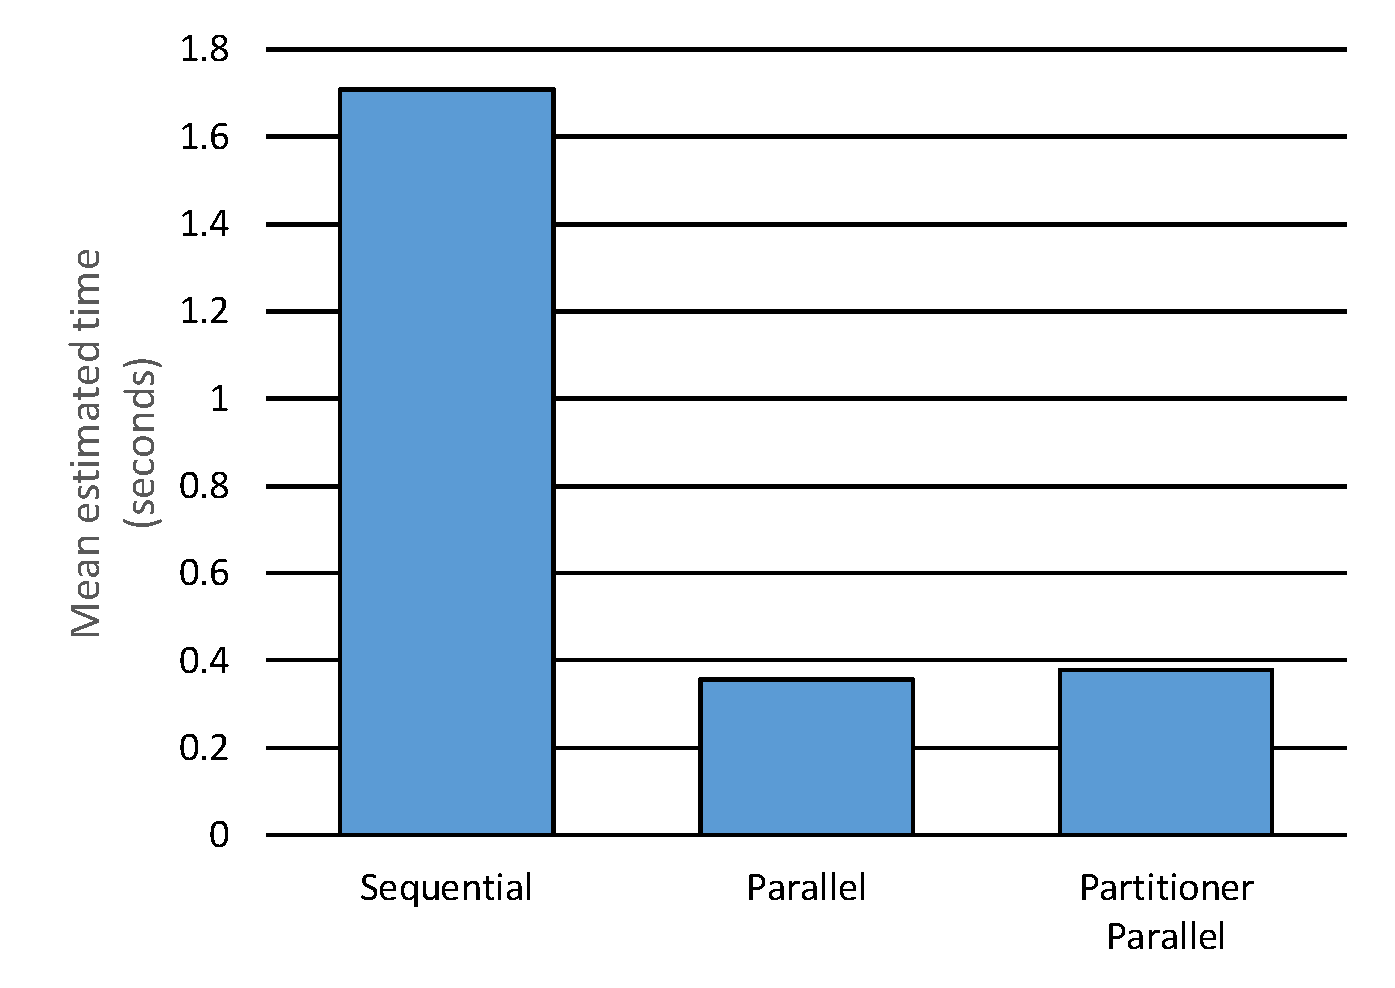
\includegraphics[width=.8\linewidth]{figures04/NugetSmall.pdf}
\caption{NuGet package ranking performance - small dataset}
\label{fig: NugetPerfSmall}
\end{figure}

\begin{figure}[htb]
\centering
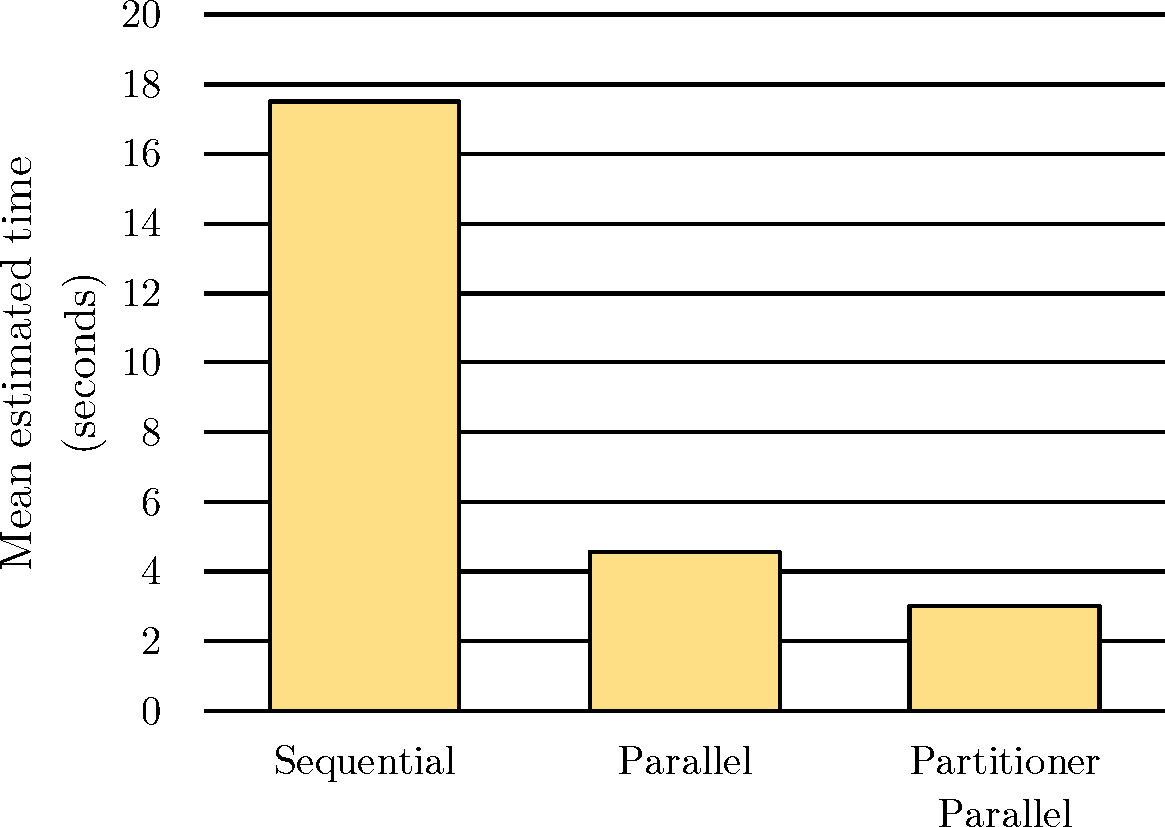
\includegraphics[width=.8\linewidth]{figures04/NugetMedium.pdf}
\caption{NuGet package ranking performance - medium dataset}
\label{fig: NugetPerfMed}
\end{figure}

\begin{figure}[htb]
\centering
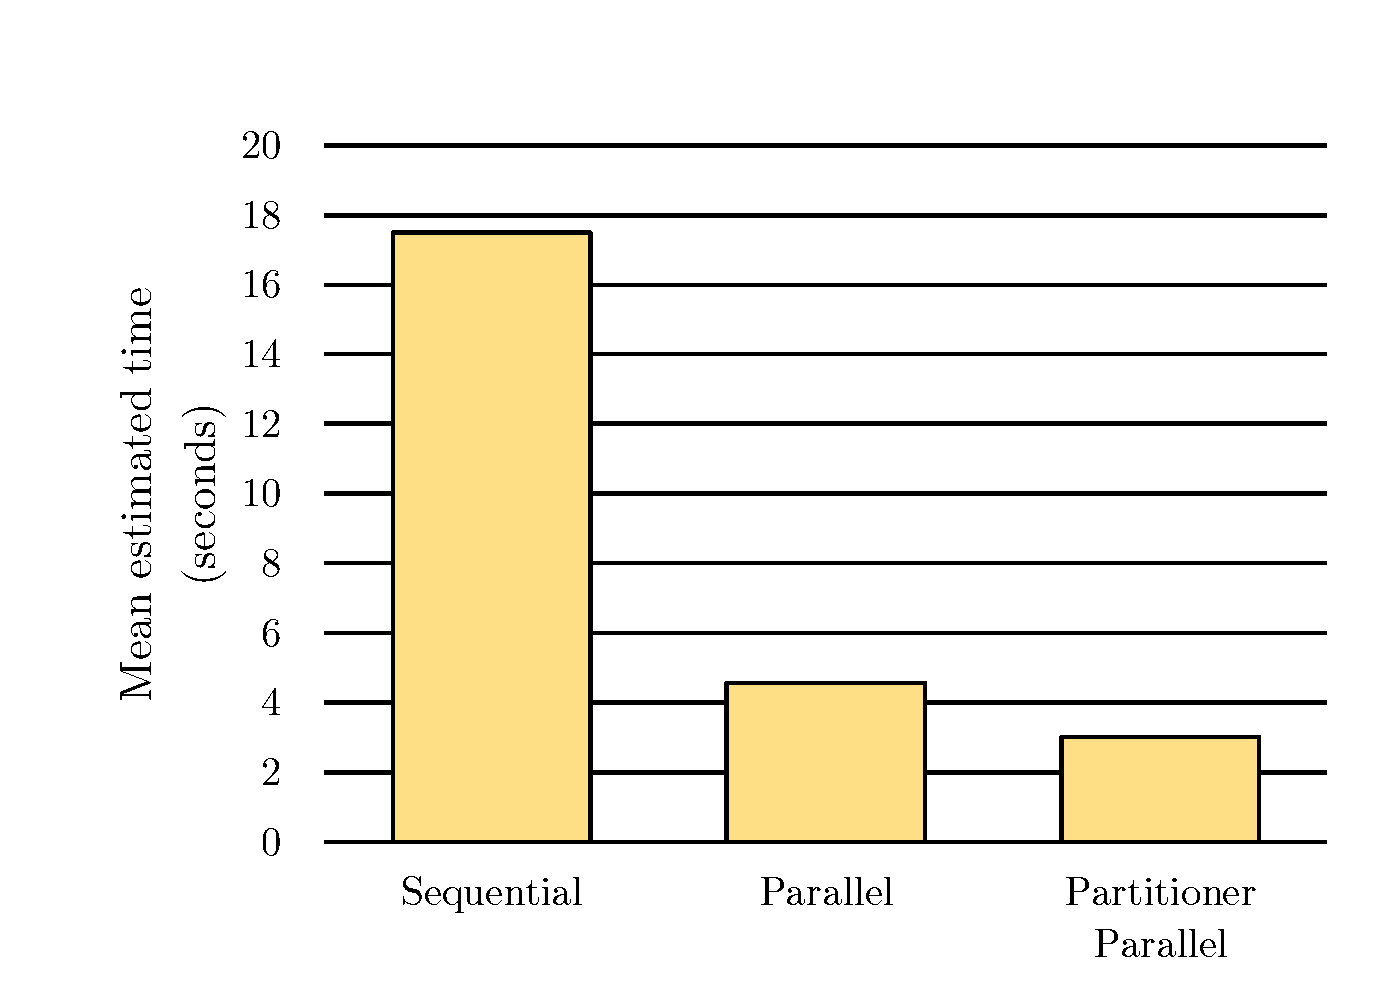
\includegraphics[width=.8\linewidth]{figures04/NugetLarge.pdf}
\caption{NuGet package ranking performance - large dataset}
\label{fig: NugetPerfLarge}
\end{figure}

\begin{figure}[htb]
\centering
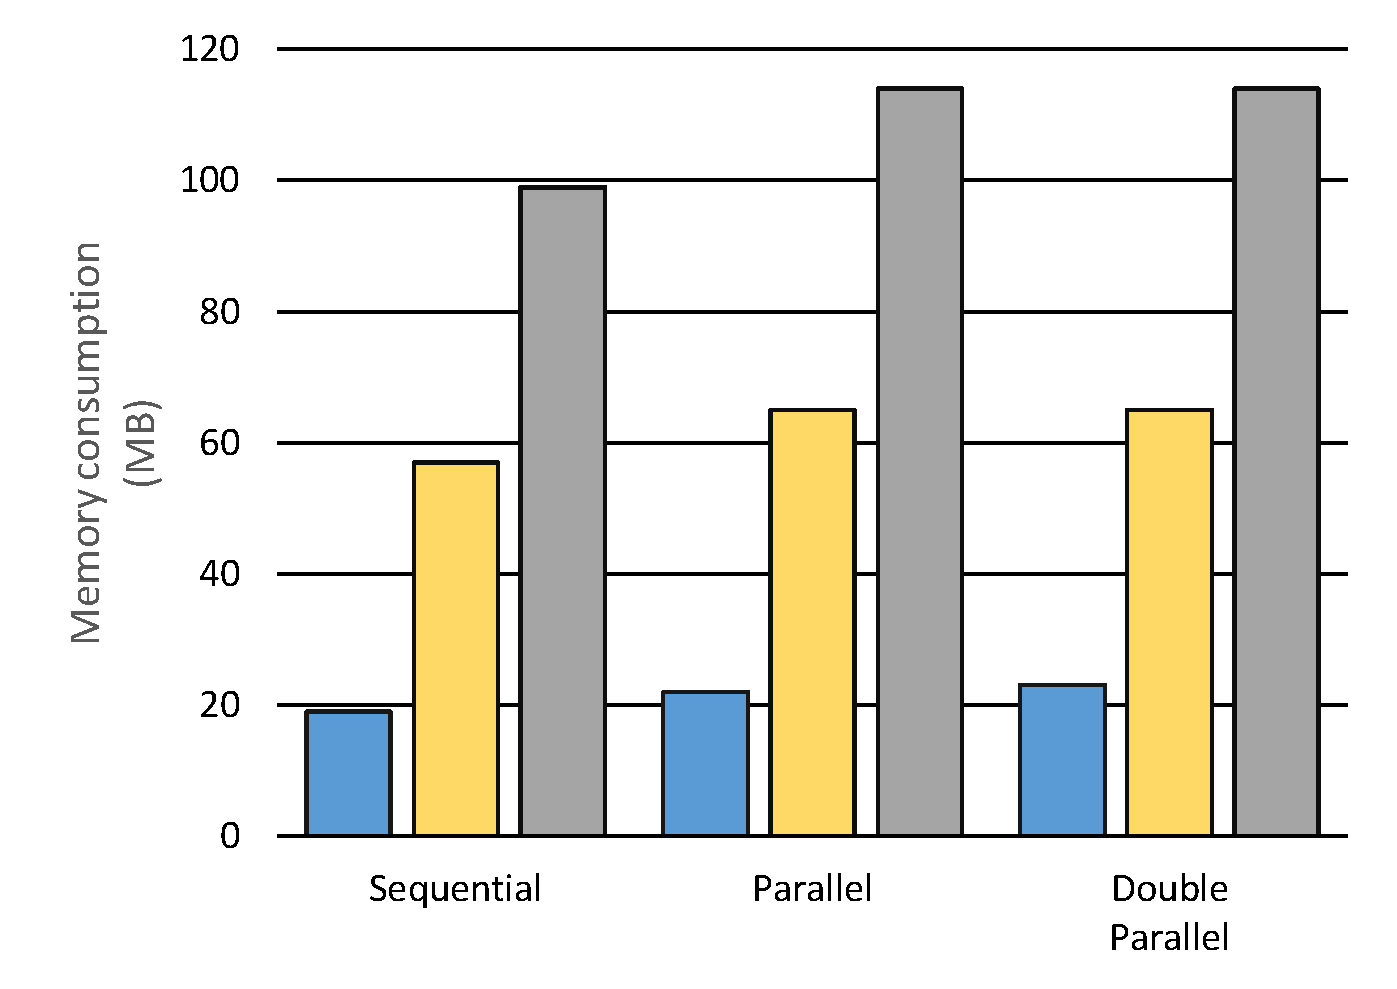
\includegraphics[width=.8\linewidth]{figures04/NugetMemory.pdf}
\caption{NuGet package ranking memory consumption}
\label{fig: NugetMemory}
\end{figure}

\begin{table}[!ht]
    \centering
    \caption{Nuget package ranking benchmarking results}
		\label{tab: NugetBenchmarking}
    \begin{tabularx}{\linewidth}{Xrrrrrrr} 
		  \toprule
			\toprule
			\bfseries Version 		&
			\bfseries Mean 	      &
			\bfseries Error       &
			\bfseries StdDev 	    &
			\bfseries Gen 0	    	&
			\bfseries Gen 1	    	&
			\bfseries Gen 2	    	&
			\bfseries Alloc.      \\ 
			&
			\bfseries {[}s{]} &
			\bfseries {[}s{]} &
			\bfseries {[}s{]} &
			&
			&
			&
			\bfseries{[}MB{]} \\			
			\midrule 
			\multicolumn{8}{c}{Small dataset} \\ 
			\midrule
			Sequential & 1.709 	& 0.004 	& 0.004 	& 2000 & 0 &    0 &	19  \\
			Parallel & 0.357 	& 0.007 	 & 0.012 	& 2000 & 1000 &	0 &	22  \\
			PartitionerParallel & 0.000  & 0.006 	& 10.33 	& 2000 & 1000 &	0 &	23  \\
			\midrule
			\multicolumn{8}{c}{Medium dataset} \\ 
			\midrule
			Sequential & 17.491    &  0.2455&	0.2296 s& 7000 & 3000 &	0 &	57  \\
			Parallel & 4.564     & 0.0684 &0.0606& 8000 & 4000 &	0 &	65 \\
			PartitionerParallel & 3.007     & 0.0577 &0.0730& 8000 & 3000 &	0 &	65  \\
			\midrule
            \multicolumn{8}{c}{Large dataset} \\ 
			\midrule
			Sequential    &      56.909&	0.6018&	0.5630&	12000 & 	5000 &	0	& 99   \\
			Paralllel     &      14.377&	0.0644&	0.0571&	14000 &	5000	 &0	& 114  \\
			PartitionerParallel &  8.428 &	0.0359&	0.0300&	14000 &	5000 &0	& 114  \\
			\bottomrule
    \end{tabularx}
\end{table}

All experiments were properly displayed and described. Next chapter will 
discuss the implications of these results and formulate a set of guidelines 
based on them. 


